Each legal, reachable board is a list of nine values $g_i\in\{-1,0,+1\}$, one per field, for circle, empty, and cross. Every board falls into one of three classes, circle win, draw, or cross win, written as target vectors $(+1,-1,-1)$, $(-1,+1,-1)$, and $(-1,-1,+1)$. Following the Meyer benchmark, unfinished games count as draws, and train and test splits are class-balanced so accuracy cannot be inflated by a dominant label. We enumerate all 5478 legal boards rather than sampling them, with the full procedure summarized in Appendix A. The label is invariant under the eight symmetries of the square, the four rotations and their reflections, which form the dihedral group $D_4$. \Cref{fig:protocol}(a) shows this directly: rotating or flipping a board never changes who has won.

To feed a board into the circuit, as in \Cref{fig:protocol}(b), we place one qubit on each field and turn each value into a rotation angle $x_i=2\pi g_i/3$ applied with a single-qubit $R_X$ gate, so circle, empty, and cross land at three evenly spaced angles:
\[
U(g)=\bigotimes_{i=0}^{8} R_X\!\left(\frac{2\pi}{3}g_i\right).
\]
Numbering the fields cyclically around the rim with the center last, as drawn in the panel, makes the board symmetry explicit. The four corners $\{0,2,4,6\}$, the four sides $\{1,3,5,7\}$, and the center $\{8\}$ are the three $D_4$ orbits: the symmetries shuffle positions within each set, but never mix one set with another.

The circuit is a stack of identical layers. Each layer re-encodes the board with $U(g)$, a data re-uploading step that lets the circuit express nonlinear functions~\cite{perezsalinas2020data}, and then applies a trainable block. Unless stated otherwise, we use $L=3$ layers with $p=2$ repetitions of the block per layer. The block is the original edge ansatz shown in \Cref{fig:protocol}(c): a single-qubit $R_YR_X$ rotation on every qubit, followed by controlled $CR_P$ entanglers on neighbouring fields and center connections.

Symmetry enters through how these gates are parameterized. Instead of giving each gate its own angle, all gates within an orbit share one trainable parameter, indicated by colour in \Cref{fig:protocol}(c): corners share one single-qubit rotation, sides another, the center keeps its own, and the $CR_P$ entanglers are tied across the orbits of the directed pairs they act on. A rotated or reflected board is then never a new, unrelated input; it permutes the same qubits and reuses the same parameters, which is precisely what makes the model equivariant. The readout follows the same geometry: we average the Pauli-$Z$ expectation over each orbit to obtain a three-number vector for corners, center, and sides, and take its largest component as the predicted class.

Because the orbits are defined by whichever symmetries we choose to enforce, we can dial the symmetry up or down without touching the wiring. For a subgroup $H\leq D_4$, parameters are tied across the orbits induced by $H$, leaving the circuit topology fixed and changing only the sharing pattern. Comparing no sharing, the two $Z_2$ subgroups, $C_4$, $D_2$, and full $D_4$ gives $204$, $108$, $126$, $60$, $78$, and $54$ trainable parameters for the edge ansatz at $L=3,p=2$, respectively; in this family, more symmetry means fewer free parameters.

The edge ansatz only couples neighbouring fields, yet a win is decided by a full three-cell line. This gap motivates the extension in \Cref{fig:protocol}(d). We add trainable gates directly on the eight winning triples, the three rows, three columns, and two diagonals shown in blue, green, and purple, using one $ZZZ$ rotation and one symmetric $CCR_Z$ interaction per triple. We test each channel on its own and together. Our main model, edge+lines, keeps the original edge ansatz and adds both line-gate channels. Crucially, these new gates are shared over the same orbits, so the model remains equivariant under the chosen subgroup. At $L=3,p=2$, the full-$D_4$ edge model has $54$ parameters and the full-$D_4$ edge+lines model has $90$, still far below the $204$ of the unshared edge baseline.

All reported runs use mean-squared error, Adam with learning rate $0.01$~\cite{kingma2015adam}, batch size 15, 30 minibatch updates per epoch, 100 epochs, fixed seed blocks, PennyLane simulation~\cite{bergholm2018pennylane}, and PyTorch optimization~\cite{paszke2019pytorch}. Exploratory runs outside this protocol are not used for any headline claim.

\begin{figure*}[!t]
\centering
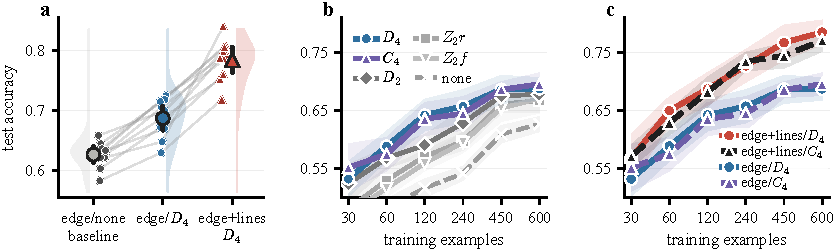
\includegraphics[width=.94\textwidth]{gfx/fig2_main_evidence}
\caption{\normalsize Main results. (a) Full $D_4$ improves over no sharing. (b) $C_4$ closely follows $D_4$ across train sizes. (c) Edge+lines gives the largest gain while preserving equivariance. Error bars are 95\% confidence intervals over seeds.}
\label{fig:main}
\end{figure*}
